\documentclass[12pt, a4paper]{article}
\usepackage[utf8]{inputenc}
\usepackage[italian]{babel}
\usepackage{amsmath, amsthm}
\usepackage{amssymb}
\usepackage{graphicx}
\usepackage{float}
\graphicspath{{img/}}
% Pacchetto per rendere l'indice cliccabile
\usepackage[hidelinks]{hyperref}

\newtheorem*{theorem}{Teorema}
\newtheorem*{definition}{Definizione}

\title{Trasformata di Fourier e ASR}
\author{Spagnoli Marcello}
\date{}

% --- CORPO ---
\begin{document}

\maketitle

% --- INDICE ---
\tableofcontents % Genera l'elenco automatico delle sezioni
\newpage         % Inizia il contenuto su una pagina nuova

\section{Introduzione}
Questo report ha il compito di tenere traccia delle conoscenze acquisite durante il tirocinio con la professoressa Lazzaro presso l'Università di Bologna per il corso di Ingegneria e Scienze Informatiche con sede a Cesena

\section{La Trasformata di Fourier}
Per arrivare alla trasformata di Fourier e alle elaborazioni che ne permettono l'uso è opportuno partire dalle basi.
L'idea alla base è quella di cambiare il dominio di rappresentazione di un segnale, nel nostro caso dal tempo alla frequenza, per cercare di cogliere caratteristiche di interesse che nel dominio iniziale non sarebbero visibili, come le lettere pronunciate da una voce o specifici strumenti musicali. \medskip

\subsection{Base di Fourier}
Partiamo nella nostra analisi considerando inizialmente segnali periodici di periodo $T > 0$: $x(t)=x(t + nT), n \in \mathbb{N}$

\begin{theorem}[Base di Fourier]

  La famiglia di funzioni $\left\{ e^{j \frac{2\pi}{T} nt} \right\}_{n \in \mathbb{Z}}$ è un sistema ortogonale e base completa di $\mathcal{L}^2([0, T])$ detta Base di Fourier
\end{theorem}

In altre parole, ogni funzione periodica può essere espressa come combinazione lineare di queste funzioni. È importante notare che si tratta di funzioni complesse, ma è possibile esprimere ogni funzione periodica anche come combinazione lineare di funzioni reali, ovvero seni e coseni.

\subsection{Serie di Fourier}
\begin{definition}[Serie di Fourier]

  Sia $x(t)$ una funzione periodica di periodo T, allora la sua serie di Fourier è data da:
  \[
    x(t) = \sum_{n=-\infty}^{\infty} c_n e^{j \frac{2\pi}{T} nt}
  \]
  dove i coefficienti $c_n$ sono dati da:
  \[
    c_n = \frac{\langle x(t), e_n \rangle}{\| e_n \|^2} = \frac{1}{T} \int_0^T x(t) e^{-j \frac{2\pi}{T} nt} \, dt
  \]

\end{definition}

Alcuni esempi visivi:

\begin{figure}[H]
  \centering
  \begin{minipage}[b]{0.40\textwidth}
    \centering
    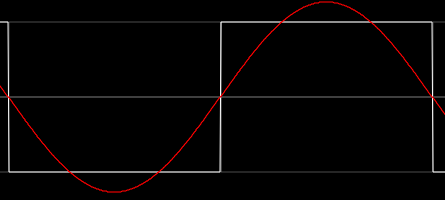
\includegraphics[width=\textwidth]{serie1.png}
  \end{minipage}
  \hspace{10pt}
  \begin{minipage}[b]{0.40\textwidth}
    \centering
    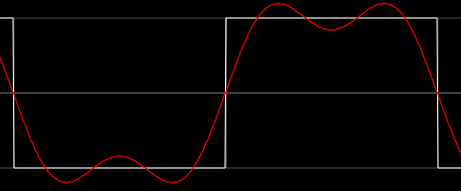
\includegraphics[width=\textwidth]{serie2.png}
  \end{minipage}

  \vspace{10pt}

  \begin{minipage}[b]{0.40\textwidth}
    \centering
    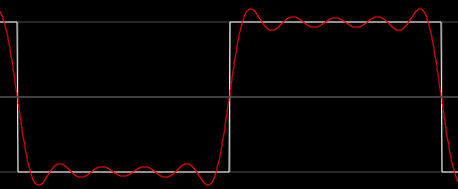
\includegraphics[width=\textwidth]{serie3.png}
  \end{minipage}
  \hspace{10pt}
  \begin{minipage}[b]{0.40\textwidth}
    \centering
    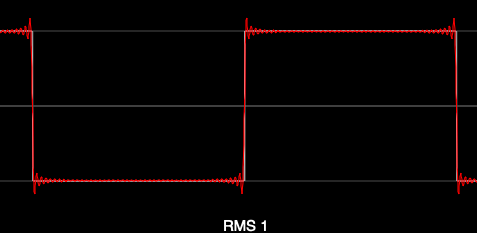
\includegraphics[width=\textwidth]{serie4.png}
  \end{minipage}
  \caption{Evoluzione della scomposizione in serie di Fourier.}
  \label{fig:serie}
\end{figure}

\subsection{Teorema di Parseval}
Il teorema di Parseval ci dice che la potenza totale di un segnale è uguale alla potenza totale dei suoi coefficienti di Fourier.

\begin{theorem}[Parseval]

  Sia $x(t) \in \mathcal{L}^2([0, T])$, allora $x(t)$ ammette sviluppo in serie di Fourier e vale la seguente uguaglianza:
  \[
    \frac{1}{T} \int_0^T |x(t)|^2 \, dt = \sum_{n=-\infty}^{\infty} |c_n|^2 < +\infty
  \]
\end{theorem}

Questo teorema ci permette di osservare che siccome $x(t)$ è a energia limitata, dal momento che appartiene a $\mathcal{L}^2([0, T])$, allora il valore di $c_n$ deve tendere a zero al crescere di n, e questo è importante per la scomposizione in frequenza di un segnale. Questo risultato infatti giustifica il fatto che ci sia una banda limitata di armoniche significative e delle code trascurabili per un'approssimazione della serie al finito.\medskip

\subsection{Trasformata di Fourier}
Tuttavia nelle applicazioni pratiche come l'ASR, i segnali che si analizzano sono aperiodici. I segnali aperiodici possono essere però visti come segnali periodici di periodo $T \to +\infty$. In questo caso però non è definita la serie di Fourier, che richiede un periodo finito. Sotto opportune ipotesi tuttavia si può ottenere una rappresentazione analoga nel dominio della frequenza grazie alla trasformata di Fourier.

\begin{theorem}[Trasformata di Fourier]

  Sia $x(t) \in \mathcal{L}^2(\mathbb{R})$ un segnale aperiodico che soddisfi le condizioni di Dirichlet:
  \begin{itemize}
    \item $x(t)$ è assolutamente integrabile in tutto $\mathbb{R}$: $\int_{-\infty}^{\infty} |x(t)| \, dt < +\infty$
    \item $x(t)$ possiede un numero finito di oscillazioni in ogni intervallo finito
    \item $x(t)$ possiede un numero finito di discontinuità in ogni intervallo finito
  \end{itemize}
  allora esiste ed è definita la trasformata di Fourier di $x(t)$, data da:
  \[
    X(f) = \mathcal{F}\{x(t)\} = \int_{-\infty}^{\infty} x(t) e^{-j 2\pi f t} \, dt
  \]
  da cui è possibile ricostruire $x(t)$ mediante l'anti-trasformata di $X(f)$:
  \[
    x(t) = \mathcal{F}^-1(X(f)) = \int_{-\infty}^{\infty} X(f) e^{j 2\pi f t} \, df
  \]
\end{theorem}

La trasformata di Fourier $\mathcal{F}(x(t))$ è di solito complessa, e si usano 2 grafici per rappresentare il contenuto in frequenza: lo spettro di ampiezza $|X(f)|$ e lo spettro di fase $\arg(X(f))$.
\medskip

Il segnale $x(t)$ è rappresentato come una somma infinita di fasori $e^{j \omega t+\theta}$ con ampiezza infinitesima $\vert X(f)\vert df$ e fase iniziale pari a $arg(X(f))$.

\subsection{Proprietà della trasformata di Fourier}

\subsubsection{Linearità}  la trasformata di Fourier è un operatore lineare, ovvero:
\begin{itemize}
  \item $\mathcal{F}\{ax(t)\} = a \mathcal{F}\{x(t)\}$
  \item $\mathcal{F}\{x(t) + y(t)\} = \mathcal{F}\{x(t)\} + \mathcal{F}\{y(t)\}$
\end{itemize}

\subsubsection{Valore in zero}
Il valore della trasformata di Fourier in zero è pari all'integrale del segnale:
\[
  X(0) = \int_{-\infty}^{\infty} x(t) \, dt
\]

\subsubsection{Traslazione temporale}
La traslazione temporale di un segnale si traduce in una modulazione complessa della sua trasformata di Fourier:
\[
  \mathcal{F}\{x(t - t_0)\} = e^{-j 2\pi f t_0} X(f)
\]

\subsubsection{Traslazione in frequenza}
La trasformata di un segnale modulato in frequenza è uguale alla traslazione in frequenza della trasformata del segnale:
\[
  \mathcal{F}\{x(t) e^{j 2\pi f_0 t}\} = X(f - f_0)
\]

\subsubsection{Simmetria}
\[
  x(t) \text{ reale e pari} \implies X(f) \text{ reale e pari}
\]
\[
  x(t) \text{ reale e dispari} \implies X(f) \text{ immaginaria pura e dispari}
\]

\subsubsection{Scaling}

La trasformata di Fourier di un segnale scalato nel tempo è data da:
\[
  \mathcal{F}\{x(at)\} = \frac{1}{|a|} X\left(\frac{f}{a}\right)
\]

\begin{figure}[h] % [h] suggerisce di metterla "qui" (here)
  \centering
  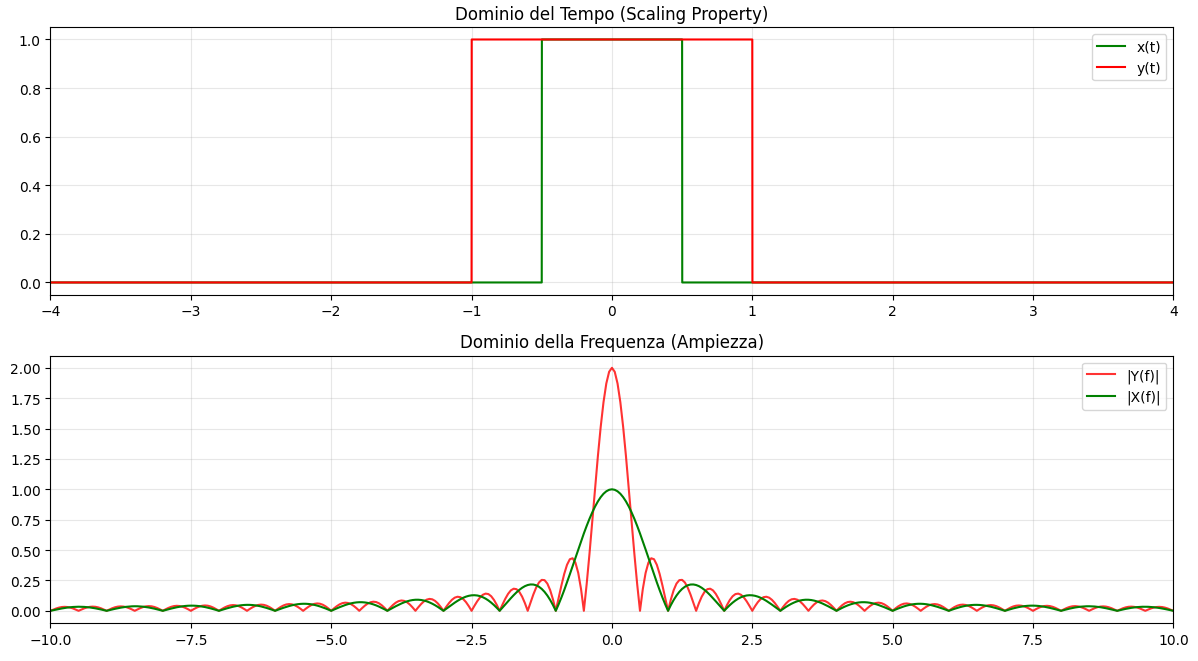
\includegraphics[width=\textwidth]{scaling.png}
  \caption{Proprietà di scalamento della Trasformata di Fourier.}
  \label{fig:scaling}
\end{figure}

\subsubsection{Derivata nel tempo}
\[
  \mathcal{F}\left\{\frac{d}{dt}x(t)\right\} = j 2\pi f X(f)
\]

\subsubsection{Integrale nel tempo}
\[
  \mathcal{F}\left\{\int_{-\infty}^{t} x(\tau) \, d\tau\right\} = \frac{X(f)}{j 2\pi f}  + \frac{X(0)\delta (f)}{2}
\]

\subsubsection{Convoluzione}

Dati due segnali $x(t)$ e $y(t)$ il prodotto di convoluzione è definito come:
\[
  x(t) * y(t) = \int_{-\infty}^{\infty} x(\tau) y(t - \tau) \, d\tau
\]
Il prodotto di convoluzione rappresenta l'effetto di filtraggio di un segnale $x(t)$ da parte di un filtro $y(t)$ e gode della proprietà commutativa ed associativa.
La trasformata di Fourier del prodotto di convoluzione è il prodotto delle trasformate dei due segnali:
\[
  \mathcal{F}\{x(t) * y(t)\} = X(f) \cdot Y(f)
\]

\subsubsection{Moltiplicazione}
\[
  \mathcal{F}\{x(t) \cdot y(t)\} = X(f) * Y(f)
\]

\subsection{Trasformata di un segnale periodico}

Posso approssimare il segnale con la serie di Fourier e poi fare la trasformata:

\[
  \mathcal{F}\{x(t)\} = \int_{-\infty}^{\infty} \sum_{n=-\infty}^{\infty} c_n e^{j 2 \pi n f_0 t} e^{-j 2\pi f t} \, dt = \sum_{n=-\infty}^{\infty} c_n \delta (f- n f_0)
\]
\[
  c_n = f_0 X(n f_0)
\]
\[
  \mathcal{F}\{x(t)\} = f_0 \sum_{n=-\infty}^{\infty} X(n f_0) \delta (f- n f_0)
\]

\subsection{DTFT}
\vspace{0.5em}
Facciamo un ulteriore passo avanti: fino a qui abbiamo considerato solamente segnali analogici, ma in realtà i segnali che si analizzano nell'ASR sono digitali, ovvero campionati e quantizzati.

Campionare un segnale significa prendere un'onda continua e 'tagliarla' a intervalli regolari. Per farlo, moltiplichiamo il segnale per una serie di impulsi: il risultato è una sequenza di punti che hanno la stessa altezza che l'onda aveva in quegli esatti istanti.

\[
  x[n] = x(t) \sum_{n=-\infty}^{+\infty} \delta(t - n T_s) = \sum_{n=-\infty}^{+\infty} x(n T_s) \delta(t - nT_s)
\]

\begin{definition}[DTFT]

  Sia $x(t)$ un segnale per cui esiste ed è definita la trasformata
  di Fourier $X(f)$. Se $x(t)$  viene campionato con intervallo di campionamento $T_s > 0$ allora il segnale ammette una rappresentazione nel dominio delle frequenze $X_s(f)$ che prende il nome di Discrete Time Fourier Transform (DTFT):
  \[
    X_s(f) = \sum_{n=-\infty}^{+\infty} x(n T_s) e^{-j 2\pi f n T_s}
  \]
  Si noti che l'espressione è analoga a una serie di Fourier con $x(n T_s)$ al posto di $c_n$ e $T_s$ al posto di $T$. La DTFT è periodica con periodo $f_s = \frac{1}{T_s}$, ovvero:
  \[
    X_s(f) = X_s(f + k f_s), \quad \forall k \in \mathbb{Z}
  \]
\end{definition}

\begin{figure}[h]
  \centering
  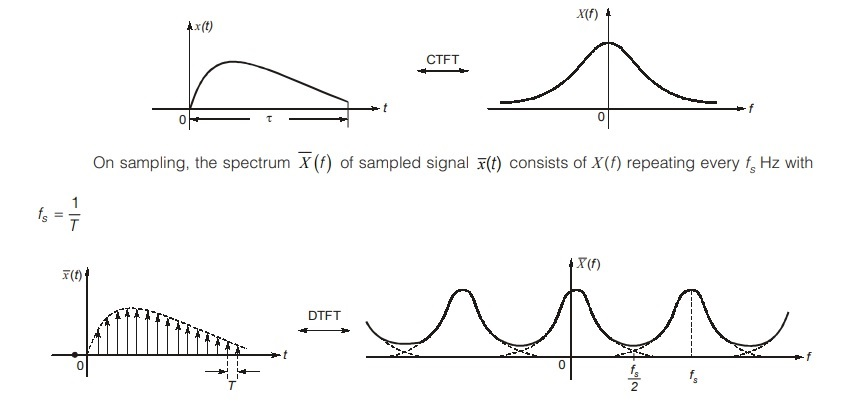
\includegraphics[width=\textwidth]{dtft.png}
  \caption{Esempio di dtft. Si noti che il segnale è periodico con periodo $f_s$.}
  \label{fig:dtft}
\end{figure}

\subsection{Campionamento di Shannon}
Ora, a partire dalla DTFT, se sono rispettate certe condizioni, si può risalire al segnale originale.

\begin{theorem}[Campionamento di Shannon]

  Sia $x(t)$ un segnale a banda limitata, ovvero esiste una frequenza $B > 0$ tale che $X(f) = 0$ per $|f| > B$. Se il segnale viene campionato con frequenza di campionamento $f_s \geq 2B$, allora l'operazione di campionamento è reversibile.
\end{theorem}

In caso in cui questa condizione sia soddisfatta, è possibile risalire al segnale originale a partire dai campioni tramite interpolazione:
\[
  x(t) = \sum_{n=-\infty}^{+\infty} x(n T_s) \text{sinc}\left(\frac{t - n T_s}{T_s}\right)
\]

Se invece $f_s < 2B$, allora si verifica un fenomeno chiamato aliasing, ovvero le ripetizioni periodiche dello spettro del segnale risultano sovrapposte, rendendo impossibile risalire al segnale originale. Ciò si vede nella figura 3.
\vspace{0.5em}

\subsection{DFT}
La DTFT tuttavia presuppone che il segnale sia infinito, ma nelle applicazioni reali si può disporre al massimo di un numero finito di $N$ valori, ovvero $x=x[n], n=0, 1, \dots, N-1$.
\vspace{0.5em}

La trasformata di Fourier per una sequenza finita di campioni prende il nome di Discrete Fourier Transform (DFT).

\begin{definition}[DFT]

  Dato un segnale discreto x[n], n=0, 1, \dots, N-1, si dice Discrete Fourier Transform di x[n] la sequenza di coefficienti di Fourier $X[k] \in \mathbb{C}^N, k=0, 1, \dots, N-1$. I coefficienti sono dati dalla formula di analisi:
  \[
    X[k] = \frac{1}{N}\sum_{n=0}^{N-1} x[n] e^{-j  \frac{2\pi}{N}kn}
  \]
\end{definition}

La DFT è un tipo di analisi di Fourier che può essere ragionevolmente implementata su un calcolatore e permette quindi data una sequenza $x$ di $N$ campioni di ottenere una sequenza $X$ di $N$ coefficienti che approssimano la trasformata di Fourier del segnale campionato.

\vspace{0.5em}
Normalmente calcolare la DFT di una sequenza di $N$ campioni richiede $O(N^2)$ operazioni, ma esistono algoritmi efficienti, come l'algoritmo Fast Fourier Transform (FFT), che permettono di calcolare la DFT in $O(N \log N)$ operazioni. La FFT sfrutta la simmetria della matrice della DFT per ridurre il numero di operazione da eseguire

\subsection{Il limite della trasformata di Fourier}
Quando si analizza un segnale con la trasformata di Fourier si assume che le sequenze che compongono il suo spettro siano presenti in ogni istante di tempo con la stessa energia: segnali di questo tipo sono detti stazionari. La maggior parte dei segnali tuttavia non lo sono: certe frequenze sono presenti solo in certi istanti, come le lettere pronunciate da una voce oppure specifici strumenti musicali all'interno di una canzone.
\vspace{0.5em}

Il limite è proprio quello di non essere in grado di cogliere nessuna informazione di localizzazione temporale del contenuto in frequenza del segnale: queste informazioni sono infatti nascoste e mescolate nella trasformata.
Queste ragioni fanno sì che per segnali non stazionari l'uso della trasformata di Fourier sia di fatto improprio

\subsection{Analisi tempo-frequenza: STFT}

Un segnale nel dominio del tempo non ha informazione di frequenza, mentre un segnale nel dominio della frequenza non ha informazione di tempo. Per superare questo limite è necessario trovare una rappresentazione che contenga sia informazione di tempo che di frequenza, ovvero una rappresentazione tempo-frequenza.
\vspace{0.5em}

Più precisamente, dato un segnale $x(t)$ si vuole dare una rappresentazione spettrale di $x(t)$ che catturi informazioni sull'evoluzione temporale del suo contenuto in frequenza.
Nella \textbf{Short-Time Fourier Transform} l'idea alla base è che un segnale non stazionario possa considerarsi stazionario su intervalli sufficientemente piccoli. A questo punto è possibile applicare la trasformata di Fourier su piccole porzioni di $x(t)$ ottenute dalla moltiplicazione con una funzione finestra $g(t)$ a supporto compatto e traslata su tutto l'asse del tempo.

\begin{definition}

  Dato un segnale $x(t)$ e una finestra $g(t)$, la Short-Time Fourier Transform (STFT) di $x(t)$ è data da:
  \[
    \text{STFT}\{x(t)\}(t, f) = \hat{X}(\tau, f) =  \int_{-\infty}^{\infty} x(\tau) \bar{g} (\tau - t) e^{-j 2\pi f \tau} \, d\tau
  \]

  $\bar{g}$ è il complesso coniugato della finestra
\end{definition}

Esiste inoltre un teorema di inversione che permette di risalire al segnale originale a partire dalla sua STFT.
\vspace{0.5em}

In generale però la STFT fornisce una rappresentazione tempo-frequenza di un segnale non stazionario $x(t)$: tramite una sequenza infinita di trasformate di Fourier la STFT fornisce le componenti in frequenza della porzione di segnale contenuta in $g(\tau - t)$ centrata in $\tau$. In questa maniera si ottengono le caratteristiche spettrali di $x(t)$ in funzione del tempo.
\vspace{0.5em}

\subsection{Spettrogramma}
La STFT è in generale una funzione complessa $\hat{X}(\tau, f)$ che viene rappresentata nel piano tempo-frequenza come spettrogramma.
\begin{definition}[Spettrogramma]

  Sia $x(t)$ un segnale che ammette una rappresentazione tempo-frequenze in termini della STFT $\hat{X}(\tau, f)$. Si definisce spettrogramma del segnale la funzione in due variabili $S: \mathbb{R}^2 \to \mathbb{R}$:
  \[
    S(t, f) = |\hat{X}(t, f)|^2
  \]
\end{definition}

\begin{figure}[ht]
  \centering
  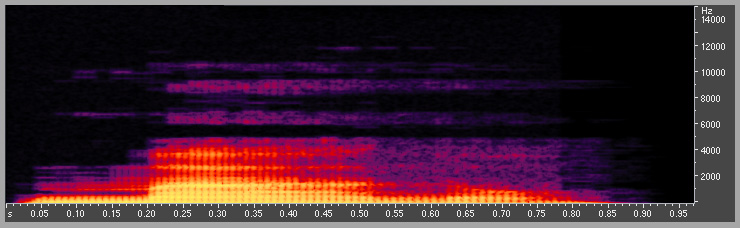
\includegraphics[width=\textwidth]{spettrogramma.png}
  \caption{Esempio di spettrogramma}
  \label{fig:spettrogramma}
\end{figure}

La scelta della finestra $g(t)$ è fondamentale per la STFT: da essa vengono univocamente determinati i parametri di risoluzione temporale e di frequenza.

\subsection{Risoluzione}
\begin{definition}[Risoluzione della finestra]

  Per un'analisi tempo-frequenza con STFT, si dice risoluzione di una finestra $g(t)$ la coppia di parametri $(\Delta t, \Delta f)$, che rappresentano rispettivamente: la distanza minima temporale tra due impulsi che possono venire discriminati nel tempo e la distanza minima in frequenza tra due sinusoidi che possono essere discriminate nel dominio delle frequenze.
\end{definition}

Questi due parametri sono legati tra loro da un principio simile a quello di indeterminazione di Heisenberg. In questo contesto è conosciuto come Limite di Gabor: egli dimostrò che per una funzione ben localizzata nel tempo non è possibile che lo spettro sia ben localizzato in frequenza, e viceversa.

Tornando alla proprietà del cambiamento di scala nel tempo della trasformata di Fourier:

\[
  \mathcal{F}\{g(at)\} = \frac{1}{|a|} G\left(\frac{f}{a}\right)
\]

Ciò significa che a una contrazione del segnale nel tempo ne corrisponde una dilatazione in frequenza della trasformata e viceversa.

È dimostrabile che il prodotto tra banda in frequenza e durata temporale di una funzione è limitato inferiormente.

\begin{theorem}[Principio di indeterminazione]

  Esiste un limite inferiore alla precisione con cui si può localizzare nel tempo una funzione e la sua trasformata di Fourier, e vale:
  \[
    \Delta _t^2 \Delta_f^2 \geq  \frac{1}{16 \pi^2}
  \]
\end{theorem}

A questo punto, avendo constatato l'impossibilità con questo approccio di avere arbitraria risoluzione sia temporale sia di frequenza, si può cercare la funzione $g(t)$ per cui il principio di indeterminazione valga con l'uguaglianza. Essa è una funzione gaussiana:
\[
  g(t) = \sqrt{\frac{a}{\pi}}e^{-at^2}
\]

per cui si ottiene
\[
  \Delta _t^2 \Delta_f^2 = \frac{1}{16 \pi^2}
\]

\begin{definition}[Trasformata di Gabor]

  La STFT di un segnale è detta Trasformata di Gabor se la funzione finestra $g(t)$ è una gaussiana $g(t) = e^{-at^2}$
\end{definition}

L'uso di una gaussiana, oltre ad avere la massima risoluzione possibile, consente anche di avere una trasformata "liscia", che non genera \emph{rippling e leakage} che andrebbero a distorcere lo spettro del segnale.

\subsection{STFT discreta}
È possibile implementare una versione discreta della STFT riconducendosi alla DFT.

In particolare si può calcolare la DFT discreta del segnale tramite una serie di DFT del segnale moltiplicato per la finestra scorrevole $g[n]$:
\[
  \hat{X}[m, k] = \sum_{n=0}^{N-1} x[n] g[n - mH] e^{-j  \frac{2\pi}{N} kn}
\]

I parametri fondamentali che definiscono questa operazione sono:

\begin{itemize}
  \item \textbf{$N$ (Window Length):} Rappresenta la lunghezza della finestra di analisi in campioni. Determina il compromesso tra risoluzione temporale e frequenziale: un $N$ elevato migliora la precisione sulle frequenze (bin più stretti) ma peggiora quella sul tempo.

  \item \textbf{$H$ (Hop-size):} È il passo di traslazione della finestra lungo il segnale. Definisce quanti campioni ci si sposta tra una DFT e la successiva.
    \begin{itemize}
      \item Se $H < N$, le finestre sono sovrapposte (\textit{overlap}).
      \item L'overlap è essenziale per compensare l'attenuazione introdotta dalla funzione $g[n]$ ai bordi. Di solito si sceglie $H = N/2$ per un buon compromesso tra riduzione dell'overlap e qualità della rappresentazione.
    \end{itemize}

  \item \textbf{$m$ (Indice Temporale):} Rappresenta l'indice della finestra corrente ($m = 0, 1, \dots, M-1$). Il tempo effettivo nel segnale originale è dato dal prodotto $t_s=\frac{mH}{f_s}$. $M$ è il numero totale di DFT calcolate. Si ottiene con la formula:
    \[ M = \left\lfloor \frac{T - N}{H} \right\rfloor \]
    dove $T$ è la durata totale del segnale. Questo garantisce che la finestra non "esca" dai confini del segnale.

  \item \textbf{$k$ e $K$ (Indice di Frequenza):} L'indice $k = 0, 1, \dots , K-1$ identifica il particolare bin di frequenza che si ottiene con $f_k = \frac{k f_s}{N}$. Poiché per segnali reali la DFT è simmetrica, ci si ferma a $K = N/2$ (frequenza di Nyquist), evitando calcoli ridondanti.
\end{itemize}

\subsection{Limiti della STFT}
I principali difetti della STFT sono:
\begin{itemize}
  \item dipendenza significativa dalla scelta della finestra $g(t)$. Essa permette di localizzare lo spettro del segnale nel tempo ma determina uno spettro che è la convoluzione tra lo spettro del segnale e lo spettro della finestra, e questo comporta uno spettro alterato.
  \item il limite di Gabor, che impone un compromesso tra risoluzione temporale e di frequenza. Non è possibile avere arbitraria risoluzione in entrambi i domini, e questo è un limite intrinseco alla STFT.
  \item Risoluzione fissa: la STFT utilizza finestre di lunghezza fissa, il che significa che la risoluzione temporale e di frequenza è costante per tutto lo spettrogramma. Questo può essere problematico per segnali con caratteristiche variabili nel tempo, come quelli vocali, dove alcune parti possono richiedere una maggiore risoluzione temporale e altre una maggiore risoluzione in frequenza.
\end{itemize}

Questo ultimo punto offre uno spunto che permette di pensare a un tipo di analisi che sfrutti una famiglia di finestre di lunghezza variabile, in modo da adattare la risoluzione alle caratteristiche del segnale in esame. Questo è il principio alla base dell'analisi wavelet dei segnali.

\section{ASR}

ASR sta per Automatic Speech Recognition, ovvero riconoscimento automatico del parlato. È considerato dagli addetti ai lavori la nuova frontiera dell'interazione uomo-macchina, e consiste nella capacità di un sistema di riconoscere e interpretare il linguaggio parlato. L'obiettivo è quello di permettere agli utenti di interagire con i dispositivi utilizzando la voce, come già accade per meccanismi di controllo vocale come Siri o strumenti di trascrizione.

\subsection{Evoluzione}
I sistemi ASR inizialmente erano sostanzialmente modulari, formati da una complessa pipeline di componenti che si occupavano di compiti specifici, come l'estrazione di caratteristiche acustiche, la modellazione acustica, la modellazione del linguaggio e la decodifica.
\begin{itemize}
  \item \textbf{Modello acustico} - Si occupa di modellare la relazione tra i suoni del parlato e le unità linguistiche (come fonemi o parole). Inizialmente venivano utilizzati modelli basati su Hidden Markov Models (HMM) e Gaussian Mixture Models (GMM) per rappresentare la variabilità acustica del parlato.
  \item \textbf{Modello di pronuncia} - ponte tra i fonemi e le parole
  \item \textbf{Modello del linguaggio} - si occupa di scegliere le parole dato il contesto, e quindi di modellare la probabilità di sequenze di parole. Inizialmente venivano utilizzati modelli basati su n-grammi, che considerano la probabilità di una parola dato un contesto limitato di parole precedenti.
\end{itemize}

Con l'avvento delle Deep Neural Network esse sono andate a sostituire i modelli basati su HMM e GMM, portando a un miglioramento significativo delle prestazioni dei sistemi ASR.
\vspace{0.5em}

Il problema di questo design modulare è che ogni componente ha bisogno di essere addestrato separatamente, e questo comporta una complessità significativa nella progettazione e nell'addestramento del sistema. Inoltre, l'ottimizzazione di ogni componente in modo indipendente non garantisce che il sistema nel suo complesso funzioni al meglio, oltre a subire particolaremente gli errori di propagazione.
\vspace{0.5em}

Per superare questi limiti, si è passati a un design \textbf{end-to-end}, in cui un singolo modello, solitamente una rete neurale profonda, viene addestrato direttamente sui dati di input (segnali audio) e output (testo trascritto). Questo approccio consente al modello di apprendere direttamente le relazioni tra i suoni del parlato e le parole, senza la necessità di componenti separate per la modellazione acustica e del linguaggio. Inoltre, l'approccio end-to-end consente di sfruttare meglio i dati disponibili, poiché il modello può apprendere direttamente dalle trascrizioni senza dover passare attraverso fasi intermedie di estrazione di caratteristiche o modellazione.
\vspace{0.5em}

Il motivo che ha permesso la transizione da design modulare a E2E è stato lo sviluppo di reti neurali capaci di imparare l'allineamento tra una sequenza di audio di lunghezza variabile e una sequenza di testo di lunghezza variabile, come le RNN, le LSTM e le Transformer. Queste architetture hanno permesso di superare il problema dell'allineamento tra input e output, che era una delle principali sfide nell'approccio modulare.
\vspace{0.5em}

\subsection{E2E paradigms}

Introduciamo ora i paradigmi base dell'approccio E2E, ovvero CTC, RNN-Transducer e Attention-based Encoder-Decoder.
\begin{itemize}
  \item \textbf{Connection Temporal Classification (CTC)} Introduce il \emph{blank token}. Usa un RNN come modello acustico che processa una sequenza audio $x=(x_1, x_2, \dots, x_n)$ e produce una sequenza di distribuzioni di probabilità $y_t$ su un alfabeto esteso che include il blank token ad ogni time step. CTC utilizza un algoritmo di programmazione dinamica per calcolare la probabilità di una trascrizione sommando su tutti i
    possibili allineamenti che, dopo aver applicato le regole di collasso (rimozione di blank consecutivi e caratteri ripetuti consecutivi),
    producono quella trascrizione target
    Un punto importante è la \emph{CTC loss function} che permette di addestrare il modello senza la necessità di allineamenti espliciti tra audio e testo, poiché considera tutte le possibili sequenze di output che possono essere mappate alla trascrizione corretta.
    \begin{itemize}
      \item \textbf{Vantaggi:} La sua \textbf{natura non-autoregressiva} fa si che la predizione a ogni step sia indipendente dalle altre. Questo permette di parallelizzare sia il training sia l'inferenza
      \item \textbf{Svantaggi:} La sua \textbf{natura non-autoregressiva} fa si che il sistema sia "semanticamente cieco": dato un contesto, un carattere dovrebbe essere più probabile di un altro, ma per la CTC non è così. Stando così le cose, è richiesto un \emph{modello del linguaggio esterno} per avere buone performance.
    \end{itemize}
  \item \textbf{Attention-Based Encoder Decoder} è composto da 2 componenti principali:
    \begin{itemize}
      \item \textbf{Encoder} - prende in input una sequenza di feature acustiche e produce una rappresentazioni intermedie $H=(h_1, h_2, \dots, h_n)$. È tipicamente una RNN piramidale o una CNN che riduce progressivamente la dimensione temporale per catturare contesto a
        lungo raggio
      \item \textbf{Decoder} - prende in input la rappresentazione intermedia $H$ e produce una sequenza di output $y=(y_1, y_2, \dots, y_m)$ un token alla volta. Il decoder è autoregressivo, ovvero a ogni step prende in input anche la predizione precedente $y_{t-1}$.
    \end{itemize}
    Il meccanismo di attenzione permette di imparare la relazione tra i frame audio e i token di output. Questi sistemi modellano la probabilità dell'output usando la chain rule: ciò permette di imparare implicitamente un modello del linguaggio a partire dai dati di training.
    Lo \textbf{Svantaggio} è che la natura autoregressiva del decoder rende il processo di inferenza sequenziale, e quindi non parallelizzabile, con un conseguente aumento dei tempi di inferenza.
  \item \textbf{RNN-Transducer} è un'architettura che combina i punti di forza di CTC e Attention-Based Encoder Decoder. È composta da 3 componenti principali:
    \begin{itemize}
      \item \textbf{Acoustic encoder} - simile a quello della Attention-Based Encoder Decoder, prende in input una sequenza di feature acustiche e produce una rappresentazione intermedia $H=(h_1, h_2, \dots, h_t)$
      \item \textbf{Prediction network} - prende in input la sequenza di token non-blank predetti fino a quel momento $y_{<t}$ e produce una rappresentazione intermedia $P=(p_1, p_2, \dots, p_u)$. Questa componente si comporta come un modello del linguaggio esterno, ma è addestrata insieme al resto del sistema, e quindi impara a modellare il linguaggio in modo specifico per il task di ASR.
      \item \textbf{Joint network} - rete feedforward che prende in input le rappresentazioni intermedie $H$ e $P$ e produce una distribuzione di probabilità sui token di output, inclusi i blank token.
    \end{itemize}
    A ogni posizione $(t, u)$ della griglia di allineamenti (dove t è il frame temporale e u la posizione nell'output), la joint network
    calcola $P(y_{u+1}|t,u)$ per il prossimo token. Se viene predetto blank, si avanza temporalmente a $(t+1,u)$, altrimenti si emette il
    simbolo e si avanza a $(t,u+1)$. Questo permette al modello di decidere dinamicamente quando emettere simboli basandosi su contesto
    acustico ed linguistico. La loss è calcolata considerando tutte le possibili sequenze di output che possono essere mappate alla
    trascrizione corretta, in modo simile alla CTC
    È un sistema adatto allo \emph{streaming}, siccome il calcolo a ogni step dipende dal frame acustico corrente e dai token predetti fino a quel momento, e non da tutta la sequenza di input o di output. Ciò garantisce una bassa latenza.
\end{itemize}
\vspace{0.5em}

Sebbene le architetture transformer-based abbiano raggiunto state-of-the-art in molti benchmark, CTC e RNN-Transducer
rimangono ampiamente utilizzati in sistemi di produzione per le loro proprietà di efficienza computazionale e bassa latenza

\begin{itemize}
  \item \textbf{Speech Transformer} - Encoder e decoder sono stack di layer multihead di feedforward e self-attention, con meccanismo di cross-attention tra encoder e decoder. La self-attention permette al modello di cogliere l'importanza degli altri frame quando si sta encodando un frame rendendo possibile modellare le dipendenze a lungo raggio. Non c'è ricorrenza, rendendo il training parallelizzabile.
  \item \textbf{Conformer} - Combina self-attention con layer convoluzionali per catturare sia le dipendenze a lungo raggio che quelle a breve raggio. Ha un modulo feed-forward, uno di multihead self-attention e un modulo convoluzionale, che vengono combinati in modo da sfruttare i punti di forza di entrambi i meccanismi. Questo approccio ibrido si è rivelato molto efficace
\end{itemize}

\subsection{Algoritmi di ricerca}

Durante l'inferenza, il modello E2E produce una distribuzione di probabilità sui token di output a ogni step. Per ottenere la trascrizione finale, è necessario utilizzare un algoritmo di ricerca che esplori lo spazio delle possibili sequenze di output e selezioni quella con la massima probabilità.

\begin{itemize}
  \item \textbf{Greedy Search} - A ogni step, si seleziona il token con la massima probabilità. È semplice e veloce, ma è subottimale
  \item \textbf{Beam Search} - Mantiene un insieme di $k$ sequenze candidate (il "beam") a ogni step. A ogni iterazione, espande tutte le sequenze nel beam con tutti i possibili token di output e seleziona le $k$ sequenze con la massima probabilità complessiva.
  \item \textbf{Shallow Fusion} - richiede un modello del linguaggio esterno. Usa una formula aggiustabile in cui si interpola linearmente la probabilità del modello del linguaggio esterno con quella del modello acustico a ogni step del beam search. In questo modo si bilancia l'importanza del contesto acustico e del contesto linguistico durante la ricerca.
\end{itemize}

\subsection{Paradigmi di training}

Il modo in cui questi modelli vengono addestrati è importante tanto quanto l'architettura stessa, e ne condiziona pesantemente le performance. I più comuni sono:
\begin{itemize}
  \item \textbf{Supervised Learning} - è l'approccio più convenzionale, che usa l'audio e la sua trascrizione. Il modello è addestrato per minimizzare una loss che misura la differenza tra la trascrizione predetta e quella corretta. Richiede un grande quantitativo di dati etichettati, che possono essere costosi da ottenere. Una tecnica molto usata per è la \textbf{data augmentation}, che consiste nel creare nuove istanze di dati manipolando quelle esistenti. \textbf{SpecAugment} è una tecnica di data augmentation specifica per i segnali audio, che consiste nell'applicare mascheramenti casuali sia nel dominio del tempo (\emph{time masking}) che in quello della frequenza (\emph{frequency masking}), oltre che deformazioni dello spettrogramma sull'asse del tempo (\emph{time warping}). Queste manipolazioni aiutano a rendere il modello più robusto a variazioni nei dati di input, migliorando le prestazioni su dati non visti durante l'addestramento ed è ormai uno standard de facto per l'addestramento di modelli ASR.
  \item \textbf{Label Smoothing} - è una tecnica di regolarizzazione che consiste nel modificare le etichette di training in modo da renderle meno "rigide". Invece di usare etichette one-hot, si usa una distribuzione di probabilità che assegna una piccola probabilità anche alle classi sbagliate. Questo aiuta a prevenire l'overfitting e a migliorare la generalizzazione del modello.
  \item \textbf{Curriculum Learning} - è un approccio di addestramento in cui il modello impara a partire da esempi più semplici e gradualmente passa a esempi più complessi. Questo approccio aiuta a migliorare la convergenza e la stabilità dell'addestramento.
  \item \textbf{Self-Supervised Learning} - Permette ai modelli di imparare da dati audio non etichettati. È un processo a 2 fasi:
    \begin{itemize}
      \item \textbf{Pre-training} - il modello è addestrato su migliaia di ore di audio non etichettato. Attraverso un encoder convoluzionale il modello impara a estrarre rappresentazioni significative dai segnali audio: un set di queste è mascherato, e a ogni step il modello deve identificare il token corretto tra un set di negative samples. In questo modo il modello impara a catturare le caratteristiche acustiche del parlato.
      \item \textbf{Fine-tuning} - Dopo il pre-training, un layer lineare viene aggiunto e il modello viene ulteriormente addestrato su un compito specifico di ASR utilizzando dati etichettati.
    \end{itemize}

    Un esempio di modello self-supervised è \textbf{Wav2Vec 2.0}, che ha dimostrato prestazioni all'avanguardia su vari benchmark di ASR, superando anche modelli addestrati in modo supervisionato su grandi quantità di dati etichettati.

  \item \textbf{Large Scale Weak Supervision} - Paradigma che fa affidamento su grandi quantità di dati reperibili in rete, anche se contengono rumore o sono corrotti in qualche maniera. L'idea è che, con un volume sufficiente di dati, il modello possa imparare a generalizzare e a estrarre informazioni utili anche da dati di bassa qualità. Questo approccio è particolarmente utile per l'ASR, dove la raccolta di grandi quantità di dati etichettati può essere costosa e laboriosa. Un esempio è \textbf{Whisper}, un modello di ASR sviluppato da OpenAI, che è stato addestrato su un vasto dataset di audio e trascrizioni raccolti da internet, dimostrando prestazioni robuste anche su dati rumorosi o con accenti diversi.
\end{itemize}

\subsection{Benchmarks}
Esistono dei benchmark standardizzati, alcuni dei quali vengono usati per valutare le prestazioni dei modelli ASR. Si dividono in monolinguistici e multilinguistici.
\begin{figure}[ht]
  \centering
  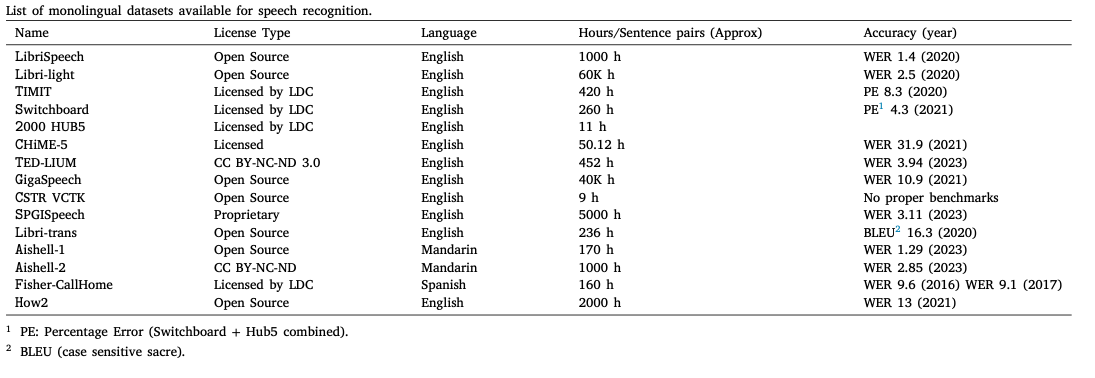
\includegraphics[width=\textwidth]{monolingual-datasets.png}
  \caption{Benchmarks monolinguistici ASR.}
  \label{fig:monolingual}
\end{figure}
\begin{figure}[ht]
  \centering
  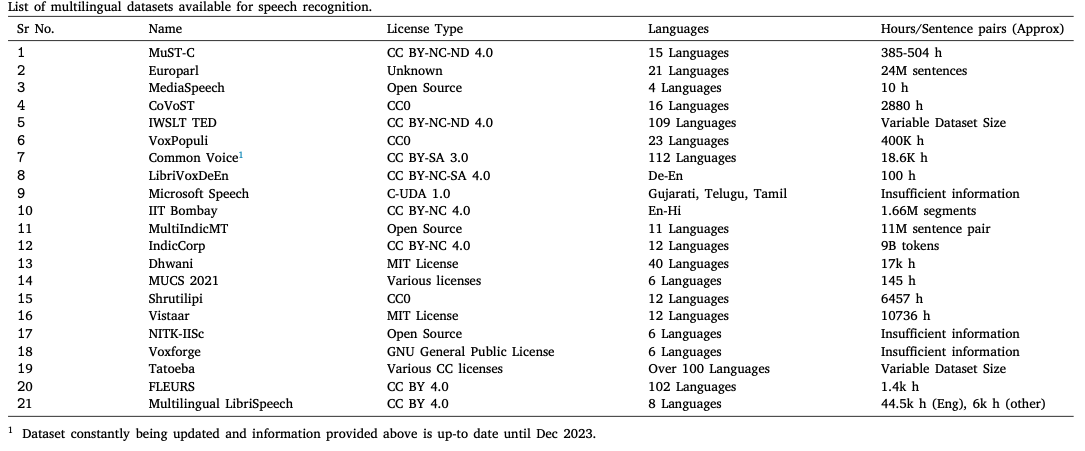
\includegraphics[width=\textwidth]{multilingual-datasets.png}
  \caption{Benchmarks multilinguistici ASR.}
  \label{fig:multilingual}
\end{figure}

Honorable mentions:
\begin{itemize}
  \item \textbf{LibriSpeech} - dataset monolinguistico in inglese, diviso in training, development e test. Il training set è ulteriormente suddiviso in "clean" e "other", a seconda della qualità dell'audio. È diventato standard de facto per la valutazione dei modelli ASR in inglese.
  \item \textbf{Switchboard} - contiene registrazioni telefoniche tra 543 persone americane che hanno accenti diversi.
  \item \textbf{TED-LIUM} - contiene registrazioni di conferenze TED, con una varietà di argomenti e stili di parlato.
  \item \textbf{Chime} - dataset focalizzato su scenari di riconoscimento del parlato in condizioni reali, con registrazioni di conversazioni in diverse condizioni acustiche.
  \item \textbf{Common Voice} - dataset multilinguistico creato da Mozilla, che contiene registrazioni vocali in diverse lingue, raccolte da volontari.
\end{itemize}

\subsection{Metriche di valutazione}
La metrica più comune per valutare le prestazioni dei modelli ASR è il Word Error Rate (WER), che misura la percentuale di parole errate nella trascrizione predetta rispetto alla trascrizione corretta. Il WER è calcolato come segue:
\[
  WER = \frac{S + D + I}{N}
\]
dove:
\begin{itemize}
  \item $S$ è il numero di sostituzioni (parole errate)
  \item $D$ è il numero di cancellazioni (parole mancanti)
  \item $I$ è il numero di inserzioni (parole aggiuntive)
  \item $N$ è il numero totale di parole nella trascrizione corretta
\end{itemize}
Chiaramente più il WER è basso, migliori sono le prestazioni del modello ASR.
\vspace{0.5em}

Un'altra metrica è il Character Error Rate (CER), che è l'analogo del WER ma che prende in considerazione i singoli caratteri.
\vspace{0.5em}

Altre metriche sono la latenza e il Real-Time Factor (RTF):
\[
  RTF =   \frac{\text{durata totale dell'audio}}{tempo di trascrizione}
\]

Tra il WER e queste ultime due metriche c'è sempre un compromesso (efficienza/velocità).

\subsection{Toolkits}
\begin{figure}[H]
  \centering
  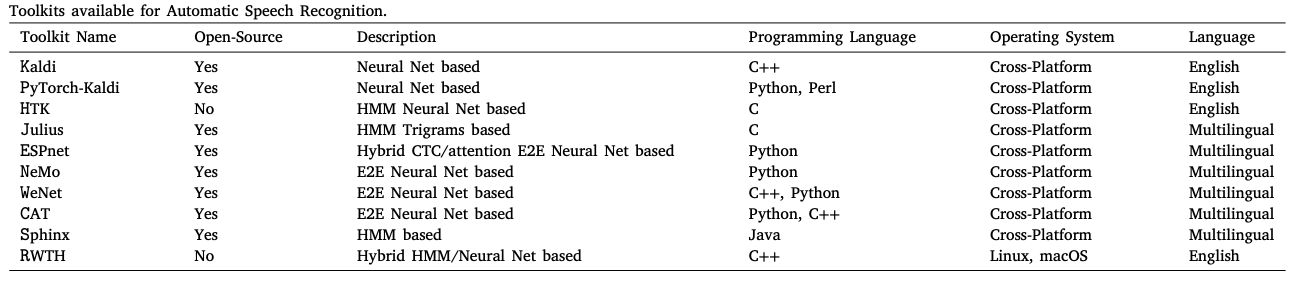
\includegraphics[width=\textwidth]{toolkits.png}
  \caption{Toolkits per ASR}
  \label{fig:toolkits}
\end{figure}

\subsection{Efficienza}
L'efficienza è molto importante per questi modelli quando poi effettivamente bisogna passare al deployment:
\begin{itemize}
  \item Molte applicazioni ASR hanno bisogno di essere Real-Time: c'è bisogno che ci sia la possibilità di fare inferenza in streaming dove il modello processa piccole porzioni di audio con delay minimo. Le \emph{RNN-T} possiedono questa caratteristica, mentre \emph{conformers e trasformers} usano una tecnica chiamata \textbf{CHUNKED ATTENTION}. L'input è diviso in chunk di lunghezza fissa e la self-attention è limitatata al chunk corrente e a un numero limitato di chunk precedenti.
    Questo genere di applicazioni richiede anche che ci sia un rilevamento della voce in modo da identificare le porzioni di audio che contengono parlato.
    \\
  \item Un altro modo di migliorare l'efficienza è la \textbf{model compression}:
    \begin{itemize}
      \item \textbf{Quantizzazione} - consiste nel ridurre la precisione dei pesi del modello, ad esempio passando da 32-bit floating point a 8-bit integer. Questo riduce la dimensione del modello e può migliorare la velocità di inferenza, soprattutto su hardware specializzato.
      \item \textbf{Pruning}:
        \begin{itemize}
          \item \textbf{Unstructured pruning} - le connessioni con pesi sotto una certa soglia sono settati a zero, creando matrici sparse
          \item \textbf{Structured pruning} - interi neuroni o layer vengono rimossi, creando un modello più piccolo e più efficiente da eseguire.
        \end{itemize}
    \end{itemize}
\end{itemize}
Queste tecniche garantiscono un buon \emph{tradeoff} tra efficienza e prestazioni, permettendo di adattare i modelli ASR a diverse esigenze e contesti di utilizzo.

\section{Implementazione della pipeline di preparazione dei dati}
Passando al lato pratico, si è implementata una pipeline di preparazione dei dati per un task di ASR, che include le seguenti fasi:

\subsection{Acquisizione del segnale audio}
Si è deciso, in quanto standard de facto, di utilizzare il dataset \textbf{LibriSpeech}, che contiene registrazioni di audiolibri in inglese. Il dataset è diviso in training, development e test set, con una suddivisione ulteriore tra "clean" e "other" a seconda della qualità dell'audio.
Con la libreria \emph{dataset} di Hugging Face si può scaricare facilmente il dataset e accedere alle registrazioni audio e alle trascrizioni corrispondenti. I dati possono essere scaricati o fruiti in modalità streaming. Ogni row ha:
\begin{itemize}
  \item \textbf{audio} - un dizionario che contiene il path del file audio, l'array dei campioni audio e la frequenza di campionamento
  \item \textbf{text} - la trascrizione del parlato contenuto nell'audio
  \item \textbf{speaker\_id} - l'identificativo del parlante
  \item \textbf{chapter\_id} - l'identificativo del capitolo dell'audiolibro
  \item \textbf{id} - un identificativo univoco per ogni registrazione
\end{itemize}

\subsection{Normalizzazione del segnale audio}
L’ampiezza del segnale viene normalizzata tra -1 e 1 per ridurre differenze di volume tra registrazioni e migliorare la stabilità dell’addestramento del modello.

\subsection{Calcolo del log-mel-spectrogram}
I modelli ASR moderni lavorano usando la scala mel. Gli umani non percepiscono le frequenze in modo lineare, ma in modo logartimico. Cìo vuol dire che la differenza tra 100 Hz e 200 Hz è percepita come più grande della differenza tra 1000 Hz e 1100 Hz, anche se in entrambi i casi la differenza è di 100 Hz. La scala mel è progettata per riflettere questa percezione umana delle frequenze, mappando le frequenze lineari a una scala logaritmica che meglio rappresenta come gli umani percepiscono i suoni.
La scala mel è una funzione a tratti definita come segue:
\[
  m(f) =
  \begin{cases}
    f & \text{se } f < 1000 \\
    2595 \cdot \log_{10}\left(1 + \frac{f}{700}\right) & \text{se } f \geq 1000
  \end{cases}
\]
\begin{figure}[H]
  \centering
  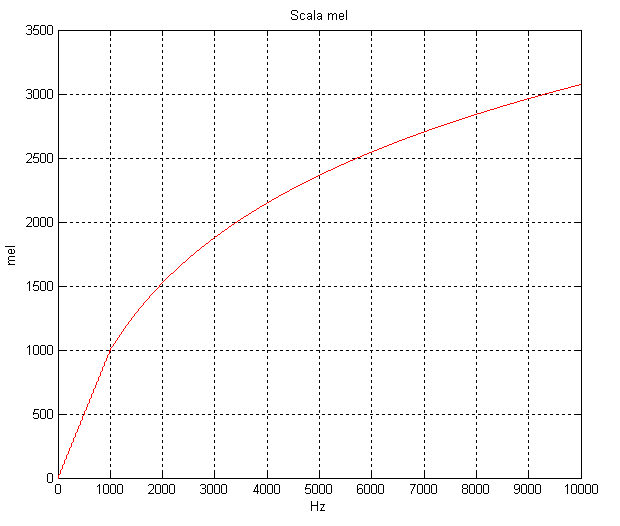
\includegraphics[width=\textwidth]{mel-scale.png}
  \caption{Grafico della scala mel}
  \label{fig:mel-scale}
\end{figure}
La filterbank Mel è un insieme di F filtri triangolari sovrapposti, distribuiti uniformemente sulla scala Mel: in quanto tali risultato più densi alle frequenze basse e più sparsi alle frequenze alte, riflettendo la percezione umana delle frequenze. Vengono applicati allo spettrogramma per ottenere uno spettrogramma mel. L'operazione è un prodotto matriciale tra la filterbank e lo spettrogramma di potenza ottenuto via STFT:
\[
  M = W \cdot S
\]

dove:
\begin{itemize}
  \item $S \in \mathbb{R}^{N \times T}$: matrice dello spettrogramma ottenuto della (STFT), con $N$ bin di frequenza e $T$ frame temporali
  \item $W \in \mathbb{R}^{F \times N}$: matrice della filterbank Mel, con $F$ filtri e $N$ bin di frequenza
  \item $M \in \mathbb{R}^{F \times T}$: matrice del mel spectrogram risultante
\end{itemize}
Ogni filtro somma le energie dei bin di frequenza che cadono nella sua banda, pesati dalla forma triangolare.
\begin{figure}[H]
  \centering
  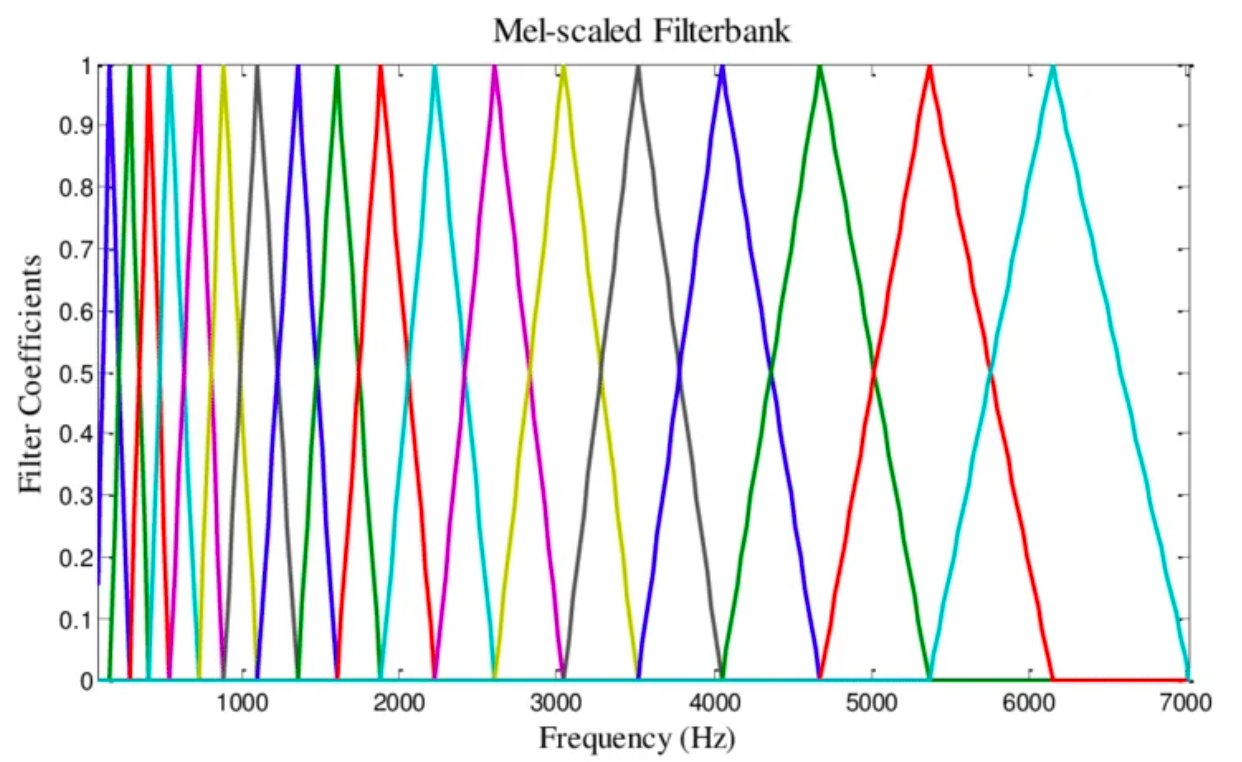
\includegraphics[width=\textwidth]{mel-filterbank.png}
  \caption{Triangoli della filterbank mel}
  \label{fig:mel-filterbank}
\end{figure}
Nel codice si usa \emph{librosa.feature.melspectrogram()} che calcola il mel spectrogram a partire dall'array dell'audio, il sampling rate e il numero di filtri mel. Dopodichè si usa \emph{librosa.power\_to\_db()} per convertire lo spettrogramma in scala logaritmica, ottenendo il log-mel-spectrogram.

\subsection{Normalizzazione delle spettrogramma}
A questo punto si fa un'altra normalizzazione: si calcola la media e la deviazione standard del log-mel-spectrogram su tutto il training set, e si normalizza ogni spettrogramma sottraendo la media e dividendo per la deviazione standard. Questo aiuta a stabilizzare l'addestramento del modello, rendendo i dati più omogenei e facilitando la convergenza.

\subsection{Costruzione vocabolario dei simboli}
Per effettuare i primi esperimenti si è costruito un vocabolario che collega ogni lettera dell'alfabeto e i segni di punteggiatura a un numero intero, in modo da poter rappresentare le trascrizioni come sequenze di interi. Dopodichè le trascrizioni degli audio disponibili sono state tradotte in usando questo vocabolario e aggiungendo il risultato in una nuova colonna di ogni row.
\end{document}
